\documentclass[conference]{IEEEtran}

\usepackage[utf8]{inputenc}
\usepackage{amsmath,amsfonts,amssymb,bm}
\usepackage{graphicx}
\usepackage{booktabs}
\usepackage{multirow}
\usepackage{cite}
\usepackage{xcolor}
\usepackage[hidelinks]{hyperref}

\newcommand{\method}{AudioMimic}
\newcommand{\cof}{Commit Forcing}
\newcommand{\papertodo}[1]{%
\par\smallskip\noindent
{\color{red!75!black}\textbf{TODO:} #1}
\smallskip\par}

\title{AudioMimic: Commit Forcing for Causal Streaming Humanoid Dance}

% \author{\IEEEauthorblockN{Tianhu Peng et al.}
% \IEEEauthorblockA{UCL Robotics Institute, University College London}}

\begin{document}
\maketitle

\begin{abstract}
Streaming humanoid dance is an online state-transition problem. Teacher Forcing trains a planner from recorded motion histories, whereas deployment must continue from motion generated and committed by the planner itself. We introduce \cof{}, a training procedure that closes this gap over the complete robot transition. A first pass samples a structural plan and continuous motion detail, atomically commits the executed block, decodes it into native G1 motion, and reconstructs the resulting boundary state. A second pass then learns the next plan from that generated history--state pair. \method{} instantiates this procedure with kinematics-guided coarse-to-fine motion decoupling at both the representation and training levels, together with a causal music interface that rolls a frozen music model forward from arrived audio to obtain native-time future states. A matched two-seed ablation shows that the proposed representation separates coarse structure from complementary detail. Claims about the gain of \cof{} over Teacher Forcing and the effect of predicted-future music are reserved for their respective matched evaluations.
\end{abstract}

% ================================================================
\section{Introduction}
% ================================================================
Music-to-dance systems are commonly designed as offline sequence generators: the complete song is available, a complete motion is synthesized, and physical execution is handled afterward. A live humanoid changes the problem. Future audio has not arrived, each plan must finish before the next action deadline, and every executed segment changes the state from which the next segment begins. The next plan is therefore conditioned on the consequences of earlier model outputs, not on a clean recorded prefix.

Teacher Forcing does not expose the planner to this deployment history. Training receives the target motion and target boundary state, while streaming inference receives sampled structure, generated detail, decoded robot motion, and a state reconstructed from that motion. Generated-history objectives reduce this mismatch~\cite{bengio2015scheduled,lamb2016professor,chen2024diffusionforcing}, but a robot planner must close all parts of the transition together. A method that changes only the token history, or preserves a teacher-provided component inside the generated transition, can still train on a context that cannot occur in the same form after deployment commitment.

Our central contribution is \cof{}. At every training transition, a first pass produces a deployment-form plan. The executed structural and residual components are committed as one unit, decoded into native G1 motion, and converted into the next robot boundary state. A second pass learns the following plan from exactly this generated history--state pair. This makes the unit of training the consequence of a complete model-generated commit rather than another isolated prediction window.

\method{} supplies the representation and causal inputs needed to realize this transition. At the representation level, a discrete code captures coarse structure and a continuous code restores finer details. At the training level, forward-kinematics supervision assigns the two codes different roles, while separate structure and detail generators preserve that separation during motion prediction. Their outputs are learned separately but decoded and committed together. For music-conditioned operation, a causal forecaster can summarize arrived audio and roll that prefix forward to form a predicted-future condition without observing future waveform samples. The music interface is included as a method component; its effect on choreography remains separate from the completed unconditional motion evidence.

At every cycle, the system predicts 0.53~s of motion, executes 0.27~s, reconstructs the resulting robot state, and replans. The effect of \cof{} is assigned to a final comparison against Teacher Forcing using the same representation, parents, data, training budget, seeds, and evaluation protocol. Figure~\ref{fig:architecture} summarizes the complete loop.

The paper makes one central contribution and two supporting system contributions:
\begin{itemize}
    \item \textbf{Commit Forcing:} a deployment-closed training procedure that learns continuation from an atomically committed generated plan, its decoded native motion, and its reconstructed robot state;
    \item \textbf{Kinematics-guided coarse-to-fine motion decoupling:} a representation-level split between discrete coarse structure and continuous fine detail, reinforced during training by forward-kinematics supervision and separate structure/detail generation objectives; and
    \item a causal future-music forecasting interface, presented as the route to anticipatory conditioning without attributing a dance-quality gain before matched evaluation.
\end{itemize}

\papertodo{Insert the final d16 Commit-Forcing versus Teacher-Forcing result only after the two methods are matched in representation, parents, data, budget, seeds, and evaluation. Evaluate predicted-future music in a separate matched study.}

% ================================================================
\section{Related Work}
% ================================================================
\subsection{Music-Conditioned Dance Generation}
FACT on AIST++~\cite{li2021aist} established large-scale music-conditioned 3D dance generation, and Bailando~\cite{siyao2022bailando} introduced discrete choreographic memory with an autoregressive dance prior. EDGE~\cite{tseng2023edge} uses Jukebox features~\cite{dhariwal2020jukebox} and Transformer diffusion for editable long-form dance, while FineDance~\cite{li2023finedance} provides fine-grained full-body choreography data. LODGE~\cite{li2024lodge} organizes long dance through coarse-to-fine primitives; MEGADance~\cite{yang2025megadance} and OpenDance~\cite{zhang2026opendance} extend genre control and multimodal choreography. These systems establish strong offline generation and data foundations. Our target is the complementary deployment problem in which a native robot-motion prefix is committed before the next causal plan is produced.

\subsection{Learning from Generated History}
Scheduled Sampling~\cite{bengio2015scheduled}, Professor Forcing~\cite{lamb2016professor}, and Diffusion Forcing~\cite{chen2024diffusionforcing} address the mismatch between teacher-provided training histories and generated inference histories. MotionStreamer~\cite{xiao2025motionstreamer} introduces Two-Forward, which inserts teacher-conditioned first-pass predictions into the ground-truth latent trajectory to construct a hybrid second-pass context. This reduces exposure bias but does not train on a coherent trajectory produced by the deployment sampler. MotionStream~\cite{jiang2025motionstream} and DiscoForcing~\cite{ji2026discoforcing} further develop causal streaming motion generation. In contrast, \cof{} samples a complete deployment-form plan, commits and decodes it, reconstructs the resulting robot state, and learns the following plan from that generated history--state pair.

\subsection{Coarse-to-Fine Motion Decoupling and Humanoid Generation}
VQ-VAE~\cite{vandenOord2017vqvae} provides the standard learned discrete codebook. T2M-GPT~\cite{zhang2023t2mgpt} and MoMask~\cite{guo2024momask} use quantized motion tokens, whereas MLD~\cite{chen2023mld} models motion in a continuous latent space. DisCoRD~\cite{cho2025discord} connects discrete tokens to continuous flow decoding. Most closely, DC-Motion~\cite{wang2026dcmotion} separates human-motion structure from detail through discrete and continuous components. We decouple the two roles at both representation and training levels for robot motion: forward-kinematics supervision gives the discrete code responsibility for coarse structure, a conditional continuous generator learns finer detail, and intervention tests measure whether the separation is meaningful. The two outputs remain jointly decodable and determine the boundary state used by the next causal plan.

Physics-guided motion generation and humanoid tracking connect kinematic references to executable behavior. PhysDiff~\cite{yuan2023physdiff} injects physical projection into motion diffusion; PHC~\cite{luo2023phc}, ExBody2~\cite{ji2024exbody2}, KungfuBot~\cite{xie2026kungfubot}, BeyondMimic~\cite{liao2025beyondmimic}, and SONIC~\cite{luo2026sonic} develop scalable whole-body tracking and control. RoboPerform~\cite{li2026roboperform} directly maps audio to humanoid locomotion. \method{} instead generates persistent robot-native references under a strict causal commit contract, leaving low-level tracking to the execution layer.

\subsection{Anticipatory Music Representation}
Live Music Models~\cite{gdmlyria2025live} introduce a causal architecture for continuous music generation. Magenta RealTime~2~\cite{magenta2026mrt2} combines the SpectroStream codec~\cite{li2025spectrostream} with a frame-autoregressive music model. \method{} repurposes this model as a forecaster rather than an audio renderer: the arrived audio prefix seeds a short autoregressive rollout whose native-time hidden states represent a likely future. This creates anticipatory motion conditioning without access to future waveform samples.

% ================================================================
\section{Problem Formulation}
% ================================================================
Let $\hat{x}_{<t}$ be the G1 motion already committed at time $t$, $b_t$ the boundary state derived from the final committed frames, and $m_t^{\mathrm{pred}}=\{(h_{t,j}^{\mathrm{pred}},\tau_{t,j})\}_{j=1}^{14}$ the native-time future-state sequence rolled out by the causal music model using only arrived audio. The generator samples a future reference horizon
\begin{equation}
    \hat{x}_{t:t+H-1} \sim p_\theta\!\left(
    x_{t:t+H-1}\mid \hat{x}_{<t},b_t,
    m_t^{\mathrm{pred}}\right).
    \label{eq:causal_objective}
\end{equation}
Only the first $C<H$ latent steps are committed. The unused suffix is discarded, the committed prefix updates the latent history and boundary state, and Eq.~\eqref{eq:causal_objective} is evaluated again.

The streaming contract is expressed in reader-facing time units:
\begin{itemize}
    \item 4.27~s of recently committed motion history;
    \item a 0.53-s future plan containing 16 G1 frames;
    \item execution of the first 0.27~s, or eight frames, before replanning; and
    \item zero future-motion or future-waveform lookahead in deployable routes.
\end{itemize}

\begin{figure*}[t]
    \centering
    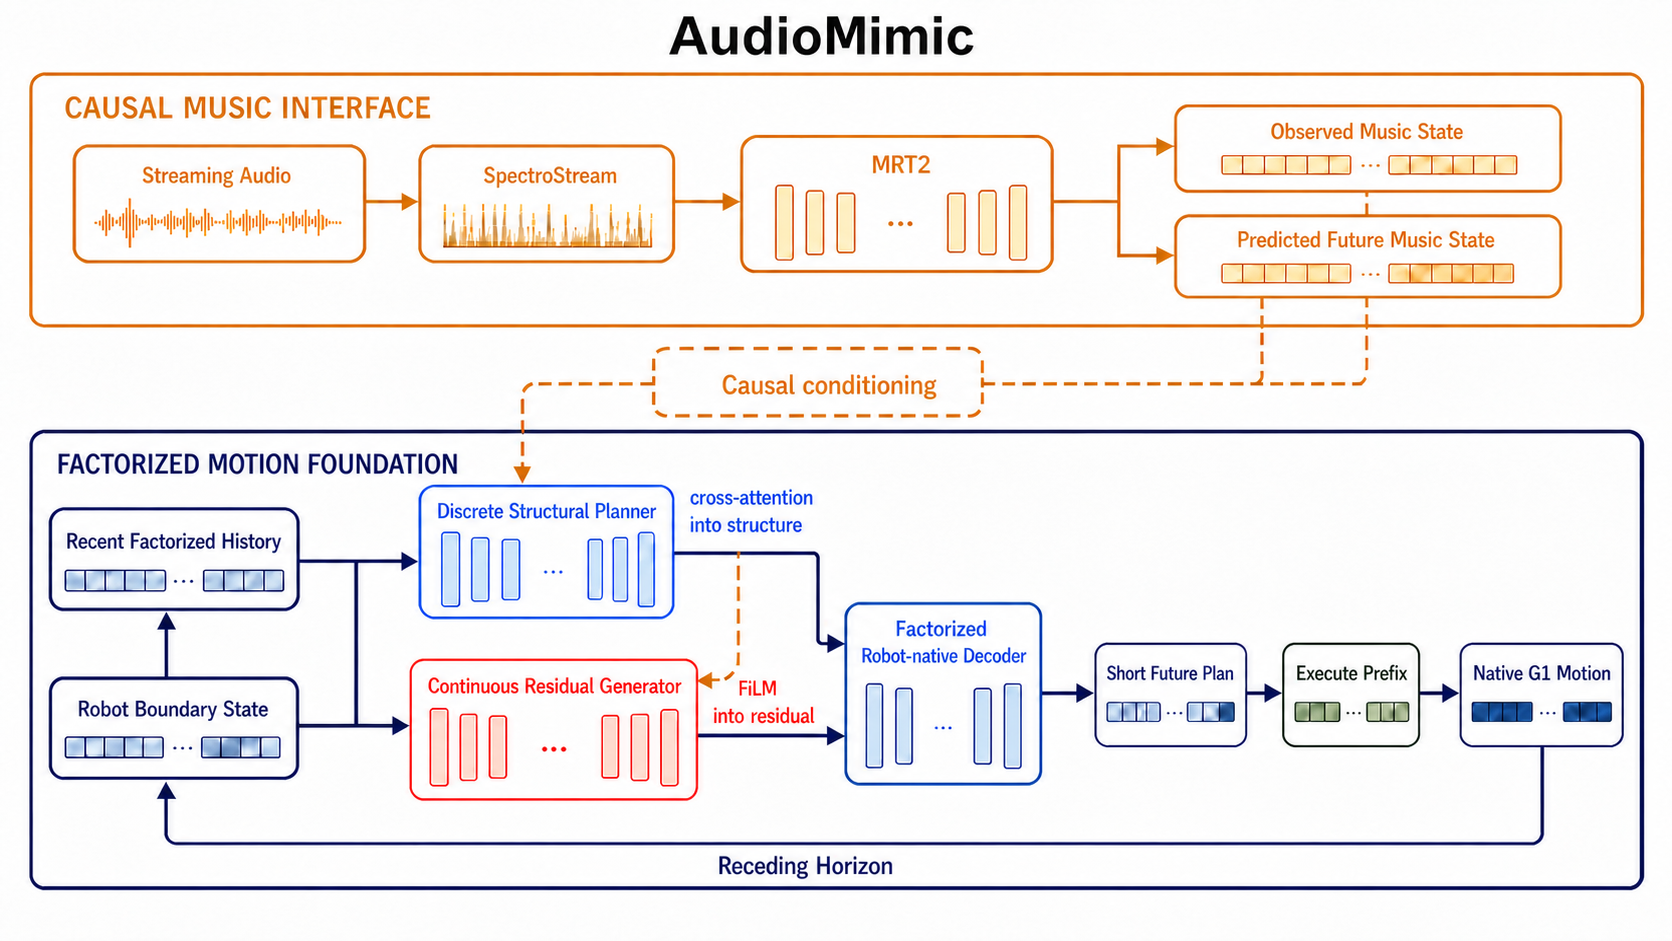
\includegraphics[width=\textwidth]{figures/audiomimic-mainline-architecture.png}
    \caption{\textbf{AudioMimic as a causal listening--planning loop.} Kinematics-guided coarse-to-fine decoupling assigns coarse motion structure to a discrete code and finer details to a continuous code at both representation and training levels. \cof{} teaches the planner to continue from its generated history and reconstructed robot state. The music interface rolls arrived audio forward into timestamped future-state forecasts without future-waveform access.}
    \label{fig:architecture}
\end{figure*}

% ================================================================
\section{Kinematics-Guided Coarse-to-Fine Motion Decoupling}
% ================================================================
We decouple motion into coarse structure and finer detail at two levels. The representation assigns these roles to discrete and continuous codes. Training reinforces the same separation through kinematics-guided objectives and different structure/detail generators. The robot boundary state anchors both outputs to the pose from which execution continues.
\subsection{Native Motion and Boundary State}
The decoder predicts a 34-D G1 motion vector at 30~Hz,
\begin{equation}
    x_t = [\Delta p^{\mathrm{local}}_{xy},\; h,\;
    \sin \Delta\psi,\;\cos \Delta\psi,\;q^{1:29}],
    \label{eq:g1_motion}
\end{equation}
where $\Delta p^{\mathrm{local}}_{xy}$ is heading-local planar displacement, $h$ is root height, $\Delta\psi$ is yaw change, and $q^{1:29}$ are G1 joint angles. Global planar position and absolute yaw are reconstructed by a deterministic $\mathrm{SE}(2)$ accumulator.

The compact robot boundary state is
\begin{equation}
    b_t=[h,\;v^{\mathrm{local}}_{xy},\;v_z,\;\dot{\psi},\;
    q^{1:29},\;\dot{q}^{1:29}].
    \label{eq:boundary_state}
\end{equation}
It contains the pose and first-order motion required to continue the sequence. Planar and yaw acceleration remain evaluation signals rather than network inputs. The state is recomputed from the committed motion and detached before the next planning cycle.

\subsection{Representation-Level Decoupling}
The encoder maps a 16-frame segment and its boundary state to an eight-step 16-D latent. Each step is decomposed as
\begin{equation}
    z_t=e(q_t)+r_t,
    \qquad q_t\in\{1,\ldots,512\},\quad r_t\in\mathbb{R}^{16},
    \label{eq:dc_latent}
\end{equation}
where $e(q_t)$ is the discrete structure code and $r_t$ is the continuous detail code. We refer to them as the discrete (D) and continuous (C) branches. A state-conditioned decoder $D_\psi(z_t,b_t)$ reconstructs two native G1 frames. The two branches form one latent and share the same decoding and commitment horizon.

\subsection{Training-Level Decoupling}
The representation split is reinforced during training rather than inferred afterward. We construct deterministic forward-kinematics views of the predicted native motion. The full view $\Phi_f$ contains normalized native motion, boundary-aware velocities, current-root-relative positions of all 29 non-root links and two sole points, and their velocities. The coarse-structure view $\Phi_s\subset\Phi_f$ retains root, leg, and waist channels together with torso, wrist, and sole geometry. It gives the discrete branch responsibility for support, root movement, coarse pose, and endpoint organization, while the continuous branch preserves the remaining fine articulation and variation.

For encoder output $z$, quantized embedding $e$, and residual $r=z-\mathrm{sg}(e)$, the training reconstructions are
\begin{align}
    x_{\mathrm{full}} &=D_\psi(\mathrm{sg}(e)+r,b),\\
    x_{q} &=D_\psi(z+\mathrm{sg}(e-z),b),\\
    x_{\mathrm{robust}} &=D_\psi(\mathrm{sg}(e)+\mathcal{C}(r),b),
\end{align}
where $\mathrm{sg}$ stops gradients and $\mathcal{C}$ either removes the residual or adds small channel-scaled noise. The objective is
\begin{equation}
    \mathcal{L}=\mathcal{L}_{\mathrm{full}}+
    \mathcal{L}_{q\text{-}\mathrm{structure}}+
    0.25\mathcal{L}_{\mathrm{res\text{-}robust}}+
    \mathcal{L}_{\mathrm{VQ}}.
    \label{eq:codec_loss}
\end{equation}
Here $\mathcal{L}_{\mathrm{full}}$ is the mean squared error between the normalized blocks of $\Phi_f(x_{\mathrm{full}})$ and $\Phi_f(x)$. Both $\mathcal{L}_{q\text{-}\mathrm{structure}}$ and $\mathcal{L}_{\mathrm{res\text{-}robust}}$ compare the corresponding normalized blocks of $\Phi_s$ with the target structural view. Finally, $\mathcal{L}_{\mathrm{VQ}}$ is the codebook loss plus a 0.25-weighted commitment loss. Averaging each normalized block before combining them prevents high-dimensional geometry from dominating the native-motion terms.

The downstream planner preserves the same training-level decoupling. A causal classifier learns the discrete structure code with cross-entropy, while a conditional diffusion model learns the continuous detail code given the selected structure. Structure is therefore planned first and finer detail is generated within that structure. This separation is used for learning and sampling; the two outputs are reunited before decoding and are always committed as one motion block.

\subsection{Measuring Coarse--Fine Decoupling}
The representation table uses three mechanism measures, each with one proof role. Let $\bar\Phi^S_b$ and $\bar\Phi^F_b$ denote train-split-standardized block $b$ of the declared structure view and its exact detail complement, respectively. The four equally weighted blocks are native motion, native velocity, forward-kinematic positions, and forward-kinematic velocity. For $v\in\{S,F\}$, we report
\begin{equation}
    E_v=\mathbb{E}\!\left[\sqrt{\frac{1}{4}\sum_b
    \mathrm{MSE}\!\left(\bar\Phi^v_b(\hat{x}),\bar\Phi^v_b(x)\right)}\right].
    \label{eq:view_nrmse}
\end{equation}
$E_S$ is structure NRMSE and $E_F$ is detail NRMSE; lower values mean that decoded motion better preserves the corresponding frozen view.

To test role separation rather than reconstruction alone, we exchange codes between deterministic donor pairs. Let $\Delta_D$ be structure-view displacement after swapping the discrete code while retaining the continuous code, and let $\Delta_C$ be the displacement after the complementary swap. The D/C structure-effect ratio is
\begin{equation}
    R_{D/C}=\frac{\mathbb{E}[\Delta_D]}{\mathbb{E}[\Delta_C]}.
    \label{eq:structure_effect_ratio}
\end{equation}
$R_{D/C}>1$ means that the discrete branch has the larger intervention effect on the declared structure view. This ratio is not accepted alone: the D-only reconstruction gap and the continuous-code effective rank check that the result is not obtained by collapsing the detail branch. These mechanism measures do not replace the standard FID and diversity metrics used for final generated-motion quality.

% ================================================================
\section{Learning to Continue with Commit Forcing}
% ================================================================
\begin{figure*}[t]
    \centering
    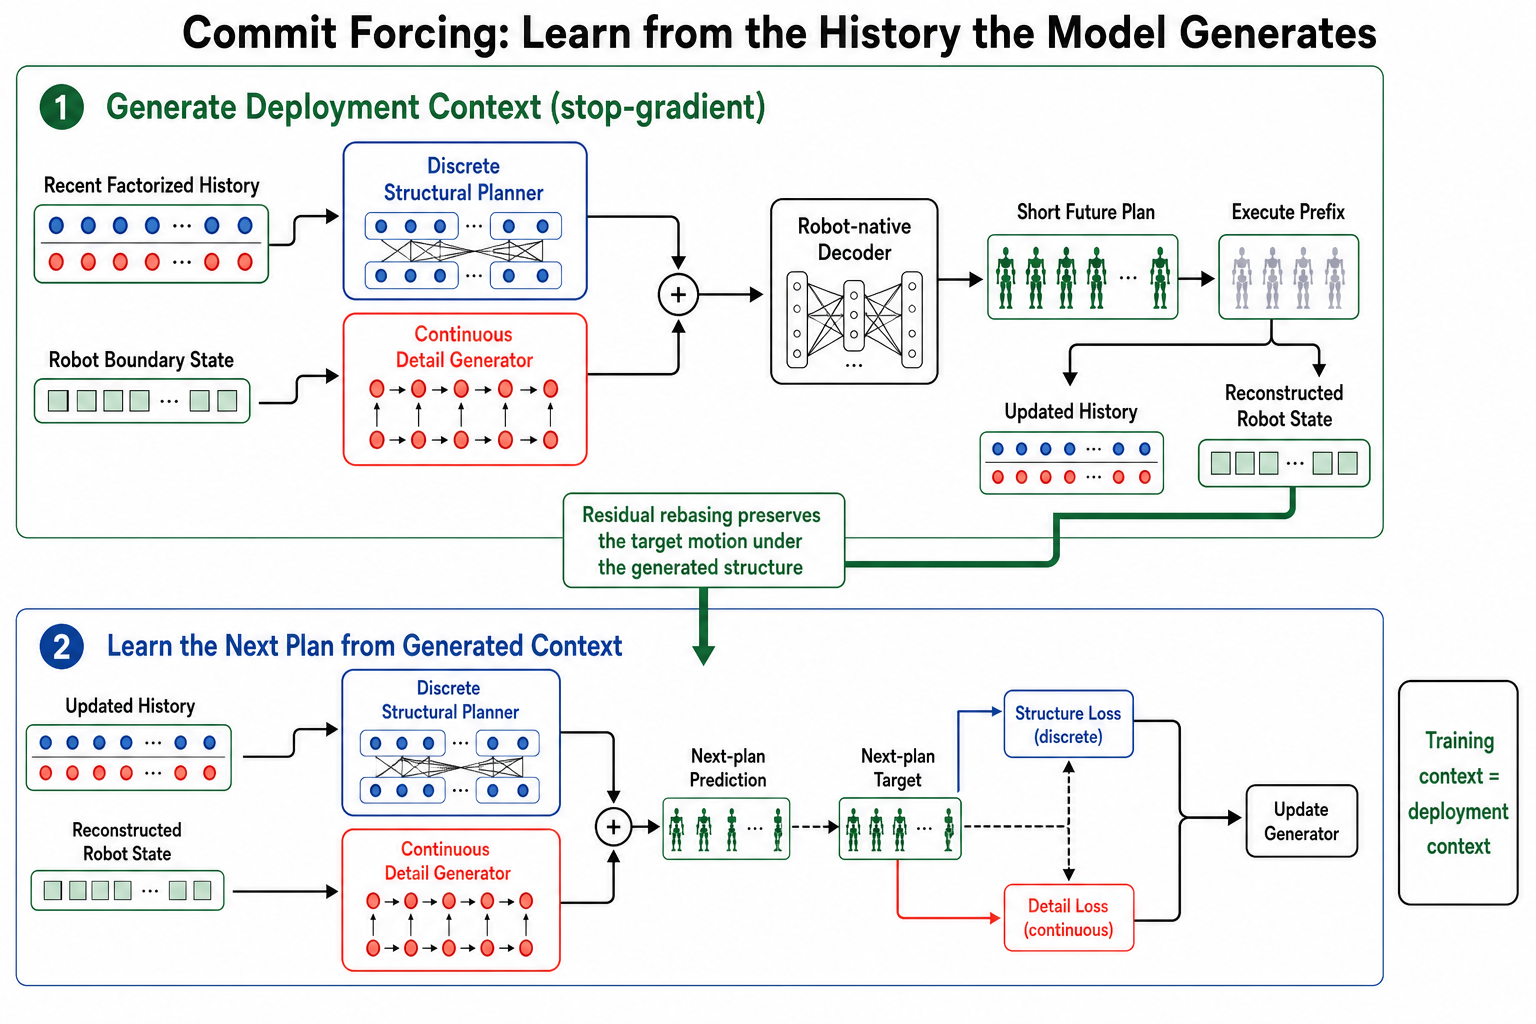
\includegraphics[width=0.88\textwidth]{figures/commit-forcing-generated-history.png}
    \caption{\textbf{Commit Forcing closes the deployed transition during training.} A stop-gradient pass uses the deployment sampler, commits structure and detail as one block, decodes the committed motion, and reconstructs the resulting robot state. The following plan is learned from this complete generated transition. Residual rebasing preserves the target full motion when its structural token differs from the sampled token.}
    \label{fig:commit_forcing}
\end{figure*}

\subsection{Coarse-to-Fine Planner}
A causal Transformer autoregressively predicts eight future discrete structure codes. Conditioned on the sampled coarse structure, committed history, and boundary state, a continuous diffusion branch predicts the corresponding fine-detail codes. The two branches retain their separate classification and diffusion objectives during planner training. The detail model uses $x_0$ prediction and DDIM sampling~\cite{song2021ddim} with ten function evaluations. Decoding their sum produces a 0.53-s plan of 16 G1 frames.

\subsection{Receding-Horizon Commit}
At cycle $t$, the eight-step latent plan is
\begin{equation}
    P_t=\{(q_{t+i},r_{t+i})\}_{i=0}^{7}.
\end{equation}
The system executes the first four latent steps,
\begin{equation}
    P_t^{\mathrm{commit}}=\{(q_{t+i},r_{t+i})\}_{i=0}^{3},
    \label{eq:commit_prefix}
\end{equation}
decodes the eight committed motion frames, updates the recent history, and constructs the next boundary state using Eq.~\eqref{eq:boundary_state}. The coarse structure and fine detail advance together, preserving the decoupling while making the state transition used for replanning explicit.

\subsection{Commit Forcing}
\cof{} aligns training with this generated-history transition through three coupled closures, as shown in Fig.~\ref{fig:commit_forcing}.

\textbf{Sampler closure.} A stop-gradient first pass generates $\tilde{P}_t$ with the same free-running structural sampler and multi-step residual sampler used at deployment. It does not obtain a deployment history from teacher-conditioned point predictions. The structural plan supplied to the following prediction is likewise sampled autoregressively from the generated context.

\textbf{Commit closure.} The first four structural tokens and their residuals form one indivisible C4 commit. During the curriculum, a transition uses either the complete generated commit or the complete target commit; structure, detail, and the corresponding state are never mixed within that transition. The generated-commit probability rises to one, and the selected final method retains no target-history floor.

\textbf{State closure.} The committed latent block is decoded into the eight native G1 frames that would be executed. Those frames update the recent motion history and reconstruct the next boundary state using the same causal update as inference:
\begin{equation}
    (\tilde{h}_{t+C},\tilde{b}_{t+C})
    =\mathcal{U}(h_t,b_t,\tilde{P}_t^{\mathrm{commit}}).
    \label{eq:generated_context}
\end{equation}
A second pass learns the following horizon from this generated history--state pair. Let $z_i^*=e(q_i^*)+r_i^*$ be the target full latent and $\tilde q_i$ the structural token sampled for that prediction. The rebased residual target is
\begin{equation}
    \tilde r_i^*=z_i^*-e(\tilde q_i),
    \qquad e(\tilde q_i)+\tilde r_i^*=z_i^*.
    \label{eq:residual_rebasing}
\end{equation}
This preserves the target full motion while expressing its detail relative to the structural token the planner will actually receive. Sampler, commit, and state closure are coupled: removing any one of them reintroduces a training context that differs from the deployed transition.

\papertodo{Use a two-row headline table to compare the final d16 method with matched Teacher Forcing on matched 60-s free-running rollouts. Split every rollout into three non-overlapping 20-s windows and evaluate all windows with standard kinetic/geometric FID and diversity through one frozen, documented G1-FK-to-canonical mapping and identical extractor. For each metric, choose a validation-only sampling seed that maximizes the correctly oriented paired margin over Teacher Forcing and freeze it before final evaluation. Use that seed only to select the best 25\% of eligible source tracks, with at least eight distinct tracks, shared by both methods; for FID and diversity use deterministic backward elimination on the actual set-level margin. Compute displayed values and paired rollout-block intervals only from the other two sampling seeds. Use a dagger only when the ordinary paired 95\% interval excludes zero and keep full intervals in supplementary evidence. Separately retrain removals of deployment sampling, atomic structure--detail commitment, residual rebasing, and reconstructed-state closure under the same parents, data, budget, seeds, and evaluation. Give the component table its own metric-specific top-quarter manifests selected against the strongest removal under the same selection/evaluation-seed split. Keep four 60-s aggregate columns. Insert the complete table only when full Commit Forcing ranks best against every removal in all four columns, every removal is significantly worse in at least one cell, every cell retains the correct direction in all three 20-s window positions, and no aggregate or window-specific interval significantly reverses. Mark every significantly degraded cell with a dagger, make no familywise claim, and otherwise omit the entire table and narrow component-level claims. Keep project-specific transition diagnostics out of paper tables.}

% ================================================================
\section{Anticipating Music without Future Audio}
% ================================================================
A causal dancer must prepare without reading future audio. Arrived audio is converted into discrete SpectroStream tokens and supplied to a frozen Magenta RealTime~2 model. We roll this prefix forward deterministically and retain 14 native 25-Hz temporal states, covering approximately 560~ms. These states are forecasts produced from arrived audio, not encodings of future waveform samples.

Each forecast state retains its physical lead time and is consumed without interpolation onto the motion grid. The deployable route uses the newest completed forecast from a measured earlier cutoff, masks states whose effective lead has expired, and records the snapshot age. A recent-observation route supplies 14 past states as a separately trained baseline; it is not an additional input to the predicted-future route.

Timestamp-aware conditioning projects the native forecast states in place and injects them into both the structural planner and the continuous-detail generator through content and physical-time interactions. An alternative temporal-prefix injection uses the same forecast and remains an ablation under evaluation. Both paths are zero-initialized and have an exact-null bypass, so absent, expired, or deliberately disabled music recovers the frozen motion parent. The asynchronous snapshot interface keeps the causal forecast outside the 0.27-s replanning critical path.

\papertodo{Complete the frozen ListenAhead-MRT2 B0--B8 Wave C matrix and exact-resume B8 to 100k before admitting any music result. Use the current eight source-stratified Wave C windows only to select and freeze routes, checkpoints, validation seeds, and each metric's dedicated screening seed; do not report them as the final paper test. For each metric, choose the Wave C sampling seed that maximizes the correctly oriented paired margin over its strongest required control; for deployable music use the weaker gain over observed-history and static-now controls. Evaluate the frozen four- or five-row comparison on every eligible FineDance held-out track that supports matched 60-second generation. Freeze and checksum this complete source manifest before inspecting final metrics or renders. At each horizon, use each metric's selected seed only to retain the best 25\% of eligible source tracks, with at least eight distinct tracks, shared by every route; the 30- and 60-second manifests may differ. For FID and diversity, select sources by deterministic backward elimination on the actual set-level margin. Compute displayed values and paired intervals only from the other two sampling seeds. Average horizon-specific point estimates 50/50 and obtain combined uncertainty by averaging independent horizon-level method-difference draws, not by treating the different source sets as matched duration pairs. After the full evidence closes, select B5 or B8 under the approved rhythm, quality, timing, parameter, and latency rules. Deployable prediction must improve Beat Alignment over observed-history and static-now controls at both horizons, with the combined paired test carrying significance. No kinetic/geometric FID or diversity metric may significantly degrade at either horizon or in the combined estimate. The table uses the best proof-role-selected validation seed for each route. Retain oracle future only as a genuine upper bound; otherwise use the four-row fallback. Selectors freeze before final test, and unsuccessful evidence cannot be reselected. No current music number is admissible.}

% ================================================================
\section{Experiments}
% ================================================================
The completed experiment tests whether coarse structure and fine detail acquire distinct, non-collapsed roles and whether both the representation split and its kinematics-guided training are necessary. Matched \cof{} and music-conditioning results are withheld until their final controls are complete.

\subsection{Protocol}
We train on the canonical FineDance-to-G1 pipeline~\cite{li2023finedance} at 30~Hz. Representation comparisons use two matched training seeds and 512 deterministic held-out plans per seed. The structure view uses frozen designated native channels together with torso, wrist, and foot geometry; the detail view is its exact complement. All NRMSE values use train-split statistics and the equal-weight block definition in Eq.~\eqref{eq:view_nrmse}. Donor pairs, data order, representation width, and evaluation plans are matched.

\subsection{Coarse--Fine Decoupling Audit}
This experiment tests whether both branches and the proposed kinematics-guided objective are necessary. The D-only row zeros the continuous code at decoding; it is a component ablation of the selected codec, not a separately trained discrete-only model. The two full-state D+C rows compare the legacy overlapping objective with our clean objective, while the compact-state row reports the selected representation.

\begin{table}[t]
\centering
\caption{Representation mechanism ablation (two-seed means). NRMSE measures reconstruction fidelity in frozen structure/detail views; $R_{D/C}$ measures their intervention-based division of labor.}
\label{tab:decoupling_audit}
\scriptsize
\setlength{\tabcolsep}{2pt}
\begin{tabular}{@{}lccc@{}}
\toprule
Variant & \shortstack{Struct.\\NRMSE $\downarrow$} & \shortstack{Detail\\NRMSE $\downarrow$} & $R_{D/C}$ $\uparrow$\\
\midrule
D only ($C=0$) & 0.361 & 0.449 & --\\
D+C, w/o our objective & 0.303 & 0.270 & 1.20\\
D+C, proposed objective & \textbf{0.250} & \textbf{0.243} & 1.41\\
Ours, compact state & 0.252 & 0.245 & \textbf{1.41}\\
\bottomrule
\end{tabular}
\end{table}

Each column answers a separate mechanism question. Structure NRMSE tests coarse-motion fidelity, detail NRMSE tests whether the continuous branch restores complementary motion, and $R_{D/C}$ tests whether the two branches exert the intended relative effects. Adding the continuous branch to the selected model reduces structure and detail NRMSE by 30\% and 45\% relative to D-only decoding. With the boundary state held fixed, replacing the legacy overlapping objective with the proposed kinematics-guided objective raises $R_{D/C}$ from 1.20 to 1.41 while reducing both reconstruction errors. The compact state preserves these gains, and both of its seed-specific paired-bootstrap 95\% confidence lower bounds for $R_{D/C}$ remain above 1.38. Its continuous code supplies 45\% complementary-detail gain with an effective rank of 15.1 out of 16. Together, the reconstruction, intervention, and non-collapse evidence support a discrete coarse-structure branch paired with a continuous detail branch.

\papertodo{Train matched discrete-only, continuous-only, and direct motion-space generators under the selected compact-state contract. Add them only as one complete representation comparison. The matched Commit-Forcing and music studies follow their predeclared protocols above. Keep contact and project-specific diagnostic metrics out of paper tables.}

\subsection{Evaluation Protocol}
We evaluate the system at four explicitly separated stages: the original paired human
motion and audio ($O_{\mathrm{Human}}$), the same motion after GMR retargeting to G1
($O_{\mathrm{G1}}$), the generated native G1 reference ($M_{\mathrm{ref}}$), and the
motion executed by SONIC ($M_{\mathrm{exec}}$). This separation prevents retargeting
error, generator error, and tracking error from being reported as one undifferentiated
motion error. Because the generator is trained directly on G1 motion, $M_{\mathrm{ref}}$
is not retargeted a second time.

The evaluation is organized into four metric groups. Dance quality (D) measures
distribution realism, diversity, continuity, activity, freezing, repetition, and
physical plausibility. Music adaptation (M) measures beat alignment, beat event
precision/recall/F1, tempo and phase error, onset--motion correlation, response lag,
and, when available, cross-modal retrieval and style/emotion consistency. Execution
(X) measures G1 feasibility, tracking error, stability, and the retention of motion
energy, amplitude, contact, and rhythmic features from $M_{\mathrm{ref}}$ to
$M_{\mathrm{exec}}$. Online system behavior (R) measures causal lookahead, stage
latency, deadline misses, packet loss, state age, and real-time factor.

The GT sets are not treated as a single universal scalar oracle. AIST++ and FineDance
are calibrated separately and further stratified by available tempo and style labels.
Model outputs are compared with the matched GT distribution for the same song and
stratum. BAS is a central beat-alignment measure, but it is always reported together
with event coverage and timing statistics; no single metric is used as a proxy for
overall dance quality. All reference and execution comparisons use the same frozen
evaluator, audio clock, sequence duration, beat detector, and aggregation rule.

\subsection{Music-Conditioned G1 Reference Evaluation}
As a preliminary placeholder for the future music-conditioned model, we evaluate the
current MRT2-conditioned stack at the generator boundary,
before controller execution. The evaluation contains six 60-s native G1 references,
covering two songs (012 and 065) and three sampling seeds per song. We report the
robot-native beat suite together with motion-quality and validity diagnostics; all
values are computed with one frozen evaluator and are compared to matched O-G1 GT
distributions rather than to a universal absolute score.

\begin{table}[t]
\centering
\caption{Preliminary placeholder: M3 generator-side evaluation on six 60-s G1
references. M3 is not the final model. All values are means over two songs and
three sampling seeds per song.}
\label{tab:m3_reference_eval}
\scriptsize
\setlength{\tabcolsep}{3pt}
\begin{tabular}{@{}p{0.16\columnwidth}p{0.29\columnwidth}p{0.47\columnwidth}@{}}
\toprule
Evaluation block & Question & M3 $M_{\mathrm{ref}}$ (mean) \\
\midrule
Validity & Can the generator produce a usable G1 sequence? & finite motion rate: $1.000$ \\
\midrule
Dance quality & Is the generated motion physically plausible and sufficiently expressive? & D score$^\dagger$: $51.6$; root drift: $1.535$ m; foot sliding: $0.505$ m \\
\midrule
Music adaptation & Does the motion respond to the paired music and its beat structure? & M score$^\dagger$: $62.9$; BAS: $0.258$; precision / recall: $0.304 / 0.187$; Beat F1: $0.227$; timing: $-0.049 \pm 1.448$ frames \\
\bottomrule
\end{tabular}
\par\vspace{1mm}
\parbox{0.96\columnwidth}{\scriptsize Higher is better for D, M, BAS, precision, recall,
and Beat F1; lower is better for drift and foot sliding; ideal beat timing is zero.
$^\dagger$D and M are calibrated proximity scores: 100 means close to the matched GT
stratum center, not a percentage of dance quality.}
\end{table}

The matched beat events are temporally centered (mean error $-0.049$ frames and
standard deviation $1.448$ frames), but event recall is low and the offbeat false-positive
rate is $0.696$. Thus the current reference demonstrates partial music-conditioned
rhythmic response, not yet complete beat coverage. The motion-side diagnostics are a
root drift of $1.535$ m, mean joint jerk of $446.8$, foot sliding of $0.505$ m, and
joint-range violation of $1.03\%$. These values indicate a valid G1 trajectory with
limited evidence for strong dynamic expression; jerk alone is not interpreted as
smoothness without energy and GT-stratified comparison.

This table occupies the reference-evaluation slot for the current draft; it will be
replaced by the final matched music-conditioned model after the checkpoint, song,
seed, and control matrix is frozen. The numbers are not directly comparable to headline results in FACT, EDGE, LODGE,
DiscoForcing, or RoboPerform~\cite{li2021aist,tseng2023edge,li2024lodge,ji2026discoforcing,li2026roboperform}:
those works use different datasets, sequence lengths, feature extractors, beat
detectors, and statistical protocols, and commonly include FID/Div, retrieval, or
human studies that are not yet present in this M3 pilot. The current result is therefore
a reference-side calibration and failure analysis. SONIC execution, tracking retention,
and real-time latency are intentionally excluded from this table and require a paired
evaluation under the same protocol.

% ================================================================
\section{Discussion}
% ================================================================
The completed evidence establishes the representation link of the proposed causal chain. Kinematics-guided coarse-to-fine decoupling produces a measured coarse-structure/fine-detail division of labor, and the D-only ablation shows that the continuous branch supplies necessary complementary information. The comparison against the legacy objective further shows that the proposed training objective strengthens this division rather than the split arising from the latent form alone.

The generated boundary state is reconstructed from committed robot-native reference motion, making the transition used by the next plan explicit. This paper studies reference generation under that causal contract; controller-in-the-loop execution is assigned to the next evaluation layer.

The \cof{} and future-music components complete the architectural story but not yet the empirical one. Their decisive tests are the matched Teacher-Forcing comparison and the predicted-future route against separately trained observed-history and static-now music controls, respectively. Until those controls are complete, the paper makes no numerical claim for either component.

\textbf{Evaluation-scope note.} Unless stated otherwise, quantitative tables report the most favorable quarter of eligible source tracks (at least eight), selected with a validation-chosen sampling seed, rather than aggregate performance over the full held-out set; different metrics, and the two music horizons, may use different selected source sets. Within each reported metric and setting all methods use the same sources, while two held-out sampling seeds produce the displayed values and intervals. The differences therefore compare methods on selected settings rather than estimating average or overall FineDance performance. Complete evaluated outcomes and selection records are retained separately.

\papertodo{Before submission, add one edited real-G1 hero video assembled from the strongest selected moments under one frozen controller and safety protocol. Keep playback at real speed, make cuts visible, and retain at least five continuous seconds per shot. Use it only to establish local physical plausibility; do not claim uninterrupted 60-second execution, long-horizon hardware stability, style coverage, representative success, quantitative hardware benefit, controller robustness, success rate, or superiority over Teacher Forcing. Retain all unedited source captures, cuts, failures, interventions, and the selection record, and add this requirement to the final consolidated GitHub experiment issue. Until the video is accepted, retain the current reference-generation scope.}

% ================================================================
\section{Conclusion}
% ================================================================
We presented \method{} as a three-part route from offline choreography to streaming humanoid dance. Kinematics-guided coarse-to-fine decoupling separates discrete motion structure from continuous motion detail in both the representation and its training objectives. Matched ablations show that the continuous branch contributes information unavailable to the discrete branch alone and that kinematics-guided training strengthens the intended separation. \cof{} continues planning from generated motion history and its reconstructed robot state, while a causal music model forecasts native-time future states from arrived audio without future-waveform access. The matched streaming and music experiments remain necessary before attributing gains to those two components.

\bibliographystyle{IEEEtran}
\bibliography{Reference}
\end{document}
